%%%%%%%%%%%%%%%%%%%%%%% file template.tex %%%%%%%%%%%%%%%%%%%%%%%%%
%
% This is a general template file for the LaTeX package SVJour3
% for Springer journals.          Springer Heidelberg 2010/09/16
%
% Copy it to a new file with a new name and use it as the basis
% for your article. Delete % signs as needed.
%
% This template includes a few options for different layouts and
% content for various journals. Please consult a previous issue of
% your journal as needed.
%
%%%%%%%%%%%%%%%%%%%%%%%%%%%%%%%%%%%%%%%%%%%%%%%%%%%%%%%%%%%%%%%%%%%
%
% First comes an example EPS file -- just ignore it and
% proceed on the \documentclass line
% your LaTeX will extract the file if required
\begin{filecontents*}{example.eps}
%!PS-Adobe-3.0 EPSF-3.0
%%BoundingBox: 19 19 221 221
%%CreationDate: Mon Sep 29 1997
%%Creator: programmed by hand (JK)
%%EndComments
gsave
newpath
  20 20 moveto
  20 220 lineto
  220 220 lineto
  220 20 lineto
closepath
2 setlinewidth
gsave
  .4 setgray fill
grestore
stroke
grestore
\end{filecontents*}
%
\RequirePackage{fix-cm}
%
%\documentclass{svjour3}                     % onecolumn (standard format)
%\documentclass[smallcondensed]{svjour3}     % onecolumn (ditto)
\documentclass[smallextended]{svjour3}       % onecolumn (second format)
%\documentclass[twocolumn]{svjour3}          % twocolumn
%
\smartqed  % flush right qed marks, e.g. at end of proof
%
\usepackage{graphicx}
%
% \usepackage{mathptmx}      % use Times fonts if available on your TeX system
%
% insert here the call for the packages your document requires
\usepackage{dsfont, amssymb,soul,xcolor, enumitem, amsmath,verbatim}
\usepackage[authoryear]{natbib}
\definecolor{linkcolor}{rgb}{0, 0, 0.54}
\usepackage[colorlinks,allcolors=linkcolor]{hyperref}
%
% please place your own definitions here and don't use \def but
\DeclareMathOperator{\E}{\mathbb{E}} % expectation
\newcommand{\Z}{\mathbb{Z}}
\newcommand{\R}{\mathbb{R}}
\newcommand{\N}{\mathbb{N}}
\newcommand{\C}{\mathbb{C}}
\renewcommand{\S}{\mathbb{S}}
\newcommand{\blank}{\makebox[1ex]{\textbf{$\cdot$}}}
\newcommand\independent{\protect\mathpalette{\protect\independenT}{\perp}}
\def\independenT#1#2{\mathrel{\rlap{$#1#2$}\mkern2mu{#1#2}}}
\renewcommand{\phi}{\varphi}
\renewcommand{\epsilon}{\varepsilon}
\newcommand*\diff{\mathop{}\!\mathrm{d}}
\newcommand{\weakly}{\rightsquigarrow}
\newcommand\smallO{\textit{o}}
\newcommand\bigO{\textit{O}}
\newcommand{\midd}{\; \middle|\;}
\newcommand{\1}{\mathds{1}}
\usepackage{ifthen} %% Empirical process with default argument
\newcommand{\G}[2][n]{
{\ensuremath{\mathbb{G}_{#1}}{\left[#2\right]}}
}
\DeclareMathOperator*{\argmin}{\arg\!\min}
\DeclareMathOperator*{\argmax}{\arg\!\max}
\newcommand{\empmeas}{\ensuremath{\mathbb{P}_n}} % empirical measure
\newcommand{\data}{\ensuremath{\mathcal{D}}}
%
% Insert the name of "your journal" with
\journalname{Lifetime Data Analysis}
%
\begin{document}

\title{The state learner -- a super learner for right-censored data
  % \thanks{Grants or other notes about the article that should go on the front
  % page should be placed here. General acknowledgments should be placed at the
  % end of the article.}
}
% \subtitle{Do you have a subtitle?\\ If so, write it here}

\titlerunning{The state learner}        % if too long for running head

\author{Blinded author}

%\authorrunning{Short form of author list} % if too long for running head

% \institute{Anders Munch \at
%               Section of Biostatistics, University of Copenhagen, Denmark \\
%               % Tel.: +123-45-678910\\
%               % Fax: +123-45-678910\\
%               \email{a.munch@sund.ku.dk}           %  \\
% %             \emph{Present address:} of F. Author  %  if needed
%               \and %
%               Thomas~A.~Gerds %
%               \at Section of Biostatistics, University of Copenhagen, Denmark}

\date{Received: date / Accepted: date}
% The correct dates will be entered by the editor


\maketitle

\begin{abstract}
  In survival analysis, prediction models are needed as stand-alone tools and in
  applications of causal inference to estimate nuisance parameters. The super
  learner is a machine learning algorithm which combines a library of prediction
  models into a meta learner based on cross-validated loss. In right-censored
  data, the choice of the loss function and the estimation of the expected loss
  need careful consideration. We introduce the state learner, a new super
  learner for survival analysis, which simultaneously evaluates libraries of
  prediction models for the event of interest and the censoring distribution.
  The state learner can be applied to all types of survival models, works in the
  presence of competing risks, and does not require a single pre-specified
  estimator of the conditional censoring distribution. We establish an oracle
  inequality for the state learner and investigate its performance through
  numerical experiments. We illustrate the application of the state learner with
  prostate cancer data, as a stand-alone prediction tool, and, for causal
  inference, as a way to estimate the nuisance parameter models of a smooth
  statistical functional.

  \keywords{Competing risks, cross-validation, loss based estimation,
    right-censored data, super learner}
% \PACS{PACS code1 \and PACS code2 \and more}
% \subclass{MSC code1 \and MSC code2 \and more}
\end{abstract}

\section{Introduction}
\label{sec:introduction}

% Medical decision making is traditionally based on the discrepancy
% between intuitive judgment and the law of chance
% \citep{redelmeier1995probability}.
% We are concerned with the statistical models that provide
% probabilistic predictions about the medical future of a patient. We
% have two different applications of these models in mind. One is as a
% stand-alone tool which predicts the likelihood of medical outcomes.
% The other is as nuisance parameter estimate
% input to an algorithm which estimates a causal target
% parameter such as an average treatment effect and depends on estimates
% of nuisance parameters such as the conditional probability of being
% uncensored.  An example of the latter is the targeted minimum loss
% based estimator \citep{rytgaard2022targeted}. In both applications,
% the models have to be learned based on available data from previous
% patients.
A super learner is a machine learning algorithm that combines a finite
set of learners into a meta learner by estimating prediction
performance in hold-out samples using a pre-specified loss function
\citep{van2007super}. When the aim is to make a prediction model,
super learners combine strong learners, such as Cox regression models
and random survival forests \citep[][Section 8.4]{gerds2021medical}.
% For targeted learning of a low dimensional
% target parameter in presence of a high-dimensional nuisance parameter,
% a super learner will usually also include the highly adaptive lasso
% \citep{van2011targeted, benkeser2016highly,van2017generally}.
While the general idea of combining strong learners based on cross-validation
stems from earlier work \citep{wolpert1992stacked,breiman1996stacked}, the
name super learner is justified by an oracle inequality
\citep{van2003unicv,vaart2006oracle}.
% The super learner is guaranteed to perform
% almost as well as the model which minimises the expected performance, i.e., the
% model we would select if we could evaluate the prediction performance in an
% infinite hold-out sample.

We define the state learner, a new super learner for right-censored data, which
simultaneously estimates the expected loss of learners of the event time
distribution and the censoring distribution. Compared to the super learners of
\cite{polley2011-sl-cens} and \cite{golmakani2020super}, the state learner
proposed here poses no restrictions on the type of learners that can be included
in the library. Compared to super learners that rely on inverse probability of
censoring weighting, censoring unbiased transformations, or pseudo-values, the
state learner does not require a pre-specified censoring distribution. Compared
to the super learners by \cite{han2021inverse} and \cite{westling2021inference},
the state learner has theoretical guarantees which these methods do not have.
% Moreover, state learner seems to be the first super learner for
% right censored data which learns the outcome and the censoring
% distribution simulaneously.

The loss function underlying the state learner operates on coarsened data. In
the right-censored survival setting the coarsened data consist of the minimum
and the order of the censoring time and the event time as well as the baseline
covariates. The state learner works by simultaneously assessing how well
learners of the event time distribution and the censoring distribution predict
the states of the coarsened data. To analyse the theoretical properties of the
state learner we focus on the discrete super learner which combines the library
of learners by picking the one that minimises the cross-validated loss
\citep{van2007super}. In the presence of competing risks, our algorithm uses
separate libraries of learners for the cumulative hazard functions for each of
the competing risks and for the censoring distribution. We show that the oracle
selector of the state learner is consistent if all libraries contain a
consistent learner and prove a finite sample oracle inequality.

The state learner algorithm can output a medical risk prediction model
\citep{gerds2021medical} which predicts the probability of an event based on
covariates in the presence of competing risks. Another important application,
which motivated our contribution, is in targeted learning where conditional
event probabilities occur as high-dimensional nuisance parameters which need to
be estimated at a certain rate \citep{van2011targeted, rytgaard2021estimation,
  rytgaard2022targeted}. The state learner is particularly well-suited for this
application as it simultaneously provides estimates for both the outcome and the
censoring, both of which are needed for targeted learning. For the asymptotic
bias term of a targeted estimator, which uses the state learner to estimate
nuisance parameters, we show that a second order product structure holds. We
illustrate both applications of the state learner with prostate cancer data
\citep{kattan2000pretreatment}.

There are many existing super learners for right-censored data. We briefly
review them here. Machine learning based on right-censored data commonly uses
the partial log-likelihood as a loss function
\citep[e.g.,][]{li2016regularized,yao2017deep,lee2018deephit,katzman2018deepsurv,gensheimer2019scalable,lee2021boosted,kvamme2021continuous}.
This loss function is also suggested for super learning with right-censored data
by \cite{polley2011-sl-cens}, where data is assumed to be observed in discrete
time. However, the partial log-likelihood loss does not work well with data
splitting (cross-validation) in continuous time. The reason is that the partial
log-likelihood loss assigns an infinite value for any learner that predicts
piece-wise constant cumulative hazard functions when there are event times in
the test set which do not occur in the learning set. This problem occurs with
prominent survival learners including the Kaplan-Meier estimator, the random
survival forest, and the semi-parametric Cox regression model and these learners
cannot be included in the library of the super learner proposed by
\cite{polley2011-sl-cens}. When a proportional hazards model is assumed, the
baseline hazard function can be profiled out of the likelihood
\citep{cox1972regression}. The cross-validated partial log-likelihood loss
\citep{verweij1993cross} has therefore been suggested as a loss function for
super learning by \cite{golmakani2020super}. This choice of loss function
restricts the library of learners to include only Cox proportional hazards
models, and hence excludes many learners such as, e.g., random survival forests,
additive hazards models, and accelerated failure time models. Other proposals
for super learning with right-censored data use an inverse probability of
censoring weighted (IPCW) loss function
\citep{graf1999assessment,van2003unicv,molinaro2004tree,keles2004asymptotically,hothorn2006survival,gerds2006consistent,gonzalez2021stacked},
censoring unbiased transformations
\citep{fan1996local,steingrimsson2019censoring}, or pseudo-values
\citep{andersen2003generalised,mogensen2013random,sachs2019ensemble}. All these
methods rely on an estimator of the censoring distribution, and their drawback
is that this estimator has to be pre-specified. An approach which avoids a
pre-specified censoring model was proposed independently by
\cite{han2021inverse} and \cite{westling2021inference}. In both articles, the
authors suggest to iterate between learning of the outcome model and learning of
the censoring model using IPCW loss functions. However, it seems that this
procedure is in general not guaranteed to converge to the true data-generating
mechanism \citep[][Appendix~A.4]{munch2024thesis}.

We introduce our notation and framework in Section~\ref{sec:framework}. In
Section~\ref{sec:super-learning} we define general super learning for
right-censored data. Section~\ref{sec:super-learner-simple} introduces the state
learner, and Section~\ref{sec:theor-results-prop} provides theoretical
guarantees. In Section~\ref{sec:targeted-learning} we discuss the use of the
state learner in the context of targeted learning. We report results of our
numerical experiments in Section~\ref{sec:numer-exper} and analyse a prostate
cancer data set in Section~\ref{sec:real-data-appl}.
Section~\ref{sec:discussion} contains a discussion of the merits and limitations
of our proposal. Proofs are given in Appendix~\ref{sec:proofs}. An
implementation of the state learner is available at
\url{https://github.com/amnudn/statelearner} along with code for reproducing our
numerical experiments.

\section{Notation and framework}
\label{sec:framework}

In a competing risk framework \citep{andersen2012statistical}, let
\( T\) be a time to event variable, \(D\in\{1,2\}\) the cause of the
event, and $X \in \mathcal{X}$ a vector of baseline covariates taking
values in a bounded subset \( \mathcal{X} \subset \R^p \),
\( p\in\N \). Let $\tau< \infty$ be the prediction horizon. We use
\( \mathcal{Q} \) to denote the collection of all probability measures
on \( [0,\tau] \times \{1,2\}\times \mathcal{X} \) such that
\( (T, D, X) \sim Q \) for some unknown \( Q \in \mathcal{Q} \). For
\(j\in\{1,2\}\), the cause-specific conditional cumulative hazard
functions are defined by
\( \Lambda_{j} \colon [0, \tau] \times \mathcal{X} \rightarrow \R_+ \)
such that
\begin{equation*}
  % \label{eq:cum-haz}
  \Lambda_{j}(t \mid x) = \int_0^t\frac{  Q(T \in \diff s, D=j \mid X=x )}{Q(T \geq s \mid X=x )}.
\end{equation*}
For ease of presentation we assume throughout that the map
\( t\mapsto \Lambda_j(t \mid x) \) is continuous for all \( x \) and
\( j \). This is not a limitation: All arguments carry over directly
to the general case. We denote by \(S\) the conditional event-free
survival function:
\begin{equation}
  \label{eq:surv-def}
  S(t \mid x)=\exp\left\{-\Lambda_{1}(t \mid x)-\Lambda_{2}(t \mid x)\right\}.
\end{equation}
Let \( \mathcal{M}_{\tau}\) denote the space of all conditional cumulative hazard
functions on \( [0,\tau] \times\mathcal{X}\). Any distribution
\( Q \in \mathcal{Q} \) can be characterised by
\begin{equation*}
  \label{eq:parametrizeQ}
  \begin{split}
    Q(\diff t,j,\diff x)=& \left\{S(t- \mid x)\Lambda_1(\diff t \mid x)H(\diff x)\right\}^{\1{\{j=1\}}}\\
                         &  \left\{S(t- \mid x)\Lambda_2(\diff t \mid x)H(\diff x)\right\}^{\1{\{j=2\}}},
  \end{split}
\end{equation*}
where \(\Lambda_{j} \in \mathcal{M}_{\tau}\) for \(j=1,2\) and \(H\) is the marginal
distribution of the covariates.

We consider the right-censored setting in which we observe the coarsened data
\(O = (\tilde{T},\tilde D, X)\), where $\tilde T = \min(T,C)$ for a
right-censoring time \(C\), $\Delta = \1{\{T \leq C\}}$, and
\(\tilde D=\Delta D\). Let \(\mathcal{P}\) denote a set of probability
measures on the sample space
\(\mathcal{O} = [0, \tau] \times \{0, 1, 2\} \times \mathcal{X}\) such
that \(O \sim P \) for some unknown \(P\in \mathcal{P}\). We assume
that the event times and the censoring times are conditionally
independent given covariates, \( T \independent C \mid X \). This
implies that any distribution \( P \in \mathcal{P} \) is characterised
by a distribution \( Q \in \mathcal{Q} \) and a conditional cumulative
hazard function for \( C \) given \( X \)
\citep[c.f.,][]{begun1983information,gill1997coarsening}. We use
\(\Gamma\in\mathcal{M}_{\tau}\) to denote the conditional cumulative hazard
function for censoring. For ease of presentation we now also assume
that \( \Gamma(\blank \mid x) \) is continuous for all \( x \). We let
\((t,x)\mapsto G(t \mid x)=\exp\left\{-\Gamma(t \mid x)\right\}\) denote the
survival function of the conditional censoring distribution. The
distribution \( P \) is characterised by
\begin{equation}\label{eq:parametrizeP}
  \begin{split}
    P(\diff t, j, \diff x) =& \left\{G(t- \mid x)S(t- \mid x)\Lambda_1(\diff t \mid x)H(\diff x)\right\}^{\1{{\{j=1\}}}}\\
                            & \left\{G(t- \mid x)S(t- \mid x)\Lambda_2(\diff t \mid x)H(\diff x)\right\}^{\1{{\{j=2\}}}}\\
                            & \left\{G(t- \mid x)S(t- \mid x)\Gamma(\diff t \mid x)H(\diff x)\right\}^{\1{{\{j=0\}}}}\\
    = & \left\{G(t- \mid x)Q(\diff t,j,\diff x)\right\}^{\1{{\{j\ne 0\}}}}\\    
                            & \left\{G(t- \mid x)S(t- \mid x)\Gamma(\diff t \mid x)H(\diff x)\right\}^{\1{{\{j=0\}}}}.
  \end{split}
\end{equation}
Hence, we may write
\( \mathcal{P} = \{ P_{Q, \Gamma} : Q \in \mathcal{Q}, \Gamma \in
\mathcal{G} \} \) for some \( \mathcal{G} \subset \mathcal{M}_{\tau} \). We
also have \(H\)-almost everywhere
\begin{equation*}
P(\tilde T>t \mid X=x) = S(t \mid x)G(t \mid x) = \exp\left\{-\Lambda_{1}(t \mid x)-\Lambda_{2}(t \mid x)-\Gamma(t \mid x) \right\}.
\end{equation*}
We further assume that there exists \(\kappa<\infty\) such that
\(\Lambda_{j}(\tau- \mid x)<\kappa \), for \(j\in\{1,2\}\), and
\(\Gamma(\tau- \mid x)<\kappa\) for almost all \(x\in\mathcal X\). Note that this
implies that \(G(\tau- \mid x)\) is bounded away from zero for almost all \(x\in\mathcal X\).
Under these assumptions, the conditional cumulative hazard functions
\(\Lambda_{j}\) and \(\Gamma\) can be identified from \(P\) by
\begin{align}
  \Lambda_{j}(t \mid x) &= \int_0^t\frac{  P(\tilde T \in \diff s, \tilde D=j \mid X=x )}{P(\tilde T \geq s \mid X=x )}, \label{eq:lambdaj}\\
  \Gamma(t \mid x) &= \int_0^t\frac{  P(\tilde T \in \diff s, \tilde D=0 \mid X=x )}{P(\tilde T \geq s \mid X=x )}\label{eq:gamma}.
\end{align}
Thus, we can consider $\Lambda_j$ and \(\Gamma\) as operators which map from
\( \mathcal{P} \) to \(\mathcal M_{\tau}\).

\section{The concept of super learning}
\label{sec:super-learning}

In survival analysis, a super learner can be used to estimate a
parameter $\Psi$ which can be identified from the observed data
distribution \(P\in\mathcal P\). In this section, to introduce the
discrete super learner and the oracle learner, we consider estimation of the
function-valued parameter \(\Psi:\mathcal P\to\mathcal M_{\tau}\), given by
\(\Psi(P)=\Lambda_j\). This parameter is identified via equation
\eqref{eq:lambdaj} on \([0,\tau]\).

As input to the super learner we need a data set
\( \data_n=\{O_i\}_{i=1}^n \) of i.i.d.\ observations from \( P \in \mathcal{P} \) and a collection of candidate
learners $\mathcal{A}$. Each learner \(a \in \mathcal{A}\) is a map
\( a \colon \mathcal{O}^n \rightarrow \mathcal{M}_{\tau}\) which takes a data
set as input and returns an estimate $a(\data_n) \in \mathcal{M}_{\tau}$ of
$\Lambda_{j}$.
% Formally, the domain of $a$ depends on \(n\) but we suppress this in the notation.
In what follows, we use the short-hand notation
\(P[f] = \int f(o) P(\diff o) \). A super learner evaluates the
performance of \(a \in \mathcal{A}\) with a loss function
\(L\colon \mathcal{M}_{\tau} \times \mathcal{O} \rightarrow \R_+\) and
estimates the expected loss \(P[L(a(\data_n), \blank)]\) using
cross-validation. Specifically, the expected loss of $a\in\mathcal A$
is estimated by splitting the data set $\data_n$ into $K$ disjoint
approximately equally sized subsets
\(\data_n^1, \data_n^2, \dots, \data_n^K \) and then calculating the
cross-validated loss
\begin{equation*}
  % \label{eq:cv-risk-est}
  \hat{R}_n(a; L) =
  \frac{1}{K}\sum_{k=1}^{K}
  % \empmeas^k{[L {(a{ (\data_n^{-k})} , \blank) }]},
  \frac{1}{| \data_n^{k} |}\sum_{O_i \in \data_n^{k}}
  L
  {
    \left(
      a{ (\data_n^{-k})}
      , O_i
    \right)
  },
  \quad \text{with} \quad
  \data_n^{-k} = \data_n \setminus \data_n^{k}.
\end{equation*}
% where \( \empmeas^{k} \) is the empirical measure of \( \data_n^{k} \). 
The subset \(\data_n^{-k}\) is referred to as the \(k\)'th training
sample, while \(\data_n^{k}\) is referred to as the \(k\)'th test or
hold-out sample.
The discrete super learner is defined as
\begin{equation*}
\hat{a}_n = \argmin_{a\in\mathcal A}\hat{R}_n(a; L).
\end{equation*}
% The final estimator of \(\Psi(P)=\Lambda_j\) is then the selected
% learner applied to the full data set, i.e., \(\hat{a}_n(\data_n)\).
The oracle learner is defined as the learner that minimises the
expected loss under the data-generating distribution \( P \),
i.e.,
\begin{equation*}
  \tilde{a}_n =
  \argmin_{a \in \mathcal{A}}
  \tilde{R}_n(a; L),
  \quad \text{with} \quad 
  \tilde{R}_n(a; L)=
  \frac{1}{K}\sum_{k=1}^{K} 
  P{
    \left[
      L
      {
        \left(
          a{ (\data_n^{-k})}
          , \blank
        \right)
      }
    \right]}
  .
\end{equation*}
Note that both the discrete super learner and the oracle learner
depend on the library of learners and on the number of folds \(K\),
and that the oracle learner is a function of the data and the unknown
data-generating distribution. However, these dependencies are
suppressed in the notation.



\section{The state learner}
\label{sec:super-learner-simple}

The main idea of the state learner is to jointly use learners for
\( \Lambda_1 \), \( \Lambda_2 \), and \( \Gamma \), and the relations in
equation~(\ref{eq:parametrizeP}), to learn a feature of the observed data
distribution \( P \). The discrete state learner ranks a tuple of learners for
the tuple of the cumulative hazard functions
\( (\Lambda_1, \Lambda_2, \Gamma) \) based on how well they jointly model the
observed data. Risk predictions can then be obtained by combining
\( \Lambda_1 \) and $\Lambda_2$ from the highest ranked tuple using a well-known
formula \citep{benichou1990estimates, ozenne2017riskregression}. To formally
introduce the state learner, we define the multi-state process
\begin{equation*}
  \eta(t) = \1\{\tilde{T} \leq t, \tilde D=1\} + 2\,\1\{\tilde{T} \leq t, \tilde
  D=2\} - \1\{\tilde{T} \leq t, \tilde D=0\},
  \quad \text{for} \quad t \in [0, \tau].
\end{equation*}
At time \(t\), we observe that each individual is in one of four mutually
exclusive states: \( 0 \), \( 1 \), \( 2 \), or \( -1 \).
The conditional distribution of the process \( \eta(t) \) given
baseline covariates \( X \) is determined by the function
\begin{equation}
  \label{eq:F-def}
  F(t, k, x) = P(\eta(t) = k \mid X=x),
\end{equation}
for all \( t \in [0,\tau] \), \( k \in \{-1,0,1,2\} \), and \( x \in \mathcal{X} \).
The function \( F \) describes the conditional state occupation probabilities of
the multi-state process \(\eta\). We construct a super learner for \( F \). The
target of this super learner is the function-valued parameter $\Psi(P) = F$
which is identified through equation~(\ref{eq:F-def}). Under conditional
independent censoring each quadruple $(\Lambda_{1}, \Lambda_{2}, \Gamma, H)$
characterises a distribution \(P\in\mathcal P\), c.f.\
equation~\eqref{eq:parametrizeP}, which in turn determines \( (F, H) \). Hence,
a learner for \( F \) can be constructed from learners for \( \Lambda_1 \),
\( \Lambda_2 \), and $\Gamma$ as follows:
\begin{equation}\label{eq:transition}
  \begin{split}
    F(t, 0, x)
    &
      = P(\tilde{T} > t \mid X= x)
      \\
      & =
      \exp{{\{-\Lambda_{1}(t \mid x)-\Lambda_{2}(t \mid x) - \Gamma(t \mid x)\}
      }},
    \\
    F(t, 1, x)
    &
      = P(\tilde{T} \leq t, \tilde{D}=1 \mid X=x)
      = \int_0^t F(s-, 0, x)  \Lambda_{1}(\diff s \mid x),
    \\
    F(t, 2, x)
    &
      = P(\tilde{T} \leq t, \tilde{D}=2 \mid X=x)
      = \int_0^t  F(s-, 0, x)  \Lambda_{2}(\diff s \mid x),
    \\
    F(t, -1, x)
    &
      = P(\tilde{T} \leq t, \tilde{D}=0 \mid X=x)
      = \int_0^t F(s-, 0, x)  \Gamma(\diff s \mid x).
  \end{split}
\end{equation}
The state learner requires three libraries of learners (c.f., Section \ref{sec:super-learning}),
\(\mathcal{A}_1\), \( \mathcal{A}_2 \), and \( \mathcal{B} \), where
\(\mathcal{A}_1\) and \( \mathcal{A}_2\) contain learners for the
conditional cause-specific cumulative hazard functions \(\Lambda_1\)
and \( \Lambda_2\), respectively, and \(\mathcal{B}\) contains
learners for the conditional cumulative hazard function of the
censoring distribution. % We further
% define \(\mathcal{H}\) as the set of all probability distributions on
% \( \mathcal{X} \) and
% \begin{equation*}
%   \mathcal{H}_n=\left\{h\colon\mathcal{O}^n\longrightarrow\mathcal{H} \midd
%     h(\data_n)=H_n = \frac 1 n \sum_{i=1}^n \delta_{X_i} \right\}
% \end{equation*}
% as the library of learners which consists of a single learner, the empirical
% distribution function.
Based on the Cartesian product of
libraries of learners for \((\Lambda_1,\Lambda_2,\Gamma)\) we construct a library
$\mathcal{F}$ of learners
for \( F \):
\begin{align*}
  \mathcal{F}(\mathcal{A}_1, \mathcal{A}_2, \mathcal{B})
  &= \{ \phi_{a_1,a_2, b} : a_1 \in \mathcal{A}_1, a_2 \in \mathcal{A}_2, b \in \mathcal{B}\},
    \intertext{where in correspondence with  the relations in equation
    \eqref{eq:transition},}
    \phi_{a_1,a_2, b}(\data_n)(t,0,x)
  &= \exp{\{-a_1(\data_n)(s \mid x)-a_2(\data_n)(s \mid x) - b(\data_n)(s \mid
    x)\} },
  \\
  \phi_{a_1,a_2, b}(\data_n)(t,1,x)
  &= \int_0^t
    \phi_{a_1,a_2, b}(\data_n)(s-,0,x)  a_1(\data_n)(\diff s \mid x),
  \\
  \phi_{a_1,a_2, b}(\data_n)(t,2,x)
  &= \int_0^t\phi_{a_1,a_2, b}(\data_n)(s-,0,x)  a_2(\data_n)(\diff s \mid x),
  \\
  \phi_{a_1,a_2, b}(\data_n)(t,-1,x)
  &= \int_0^t \phi_{a_1,a_2, b}(\data_n)(s-,0,x)  b(\data_n)(\diff s \mid x).
\end{align*}
To evaluate how well a function \( F \) predicts the observed
multi-state process we use the integrated Brier score
\( \bar B_\tau( F,O) = \int_0^{\tau} B_t(F,O) \diff t \), where \( B_t \) is the
Brier score \citep{brier1950verification} at time \( t \in [0, \tau] \),
\begin{equation*}
  B_t(F,O) = \sum_{j=-1}^{2}
  \left(
      F(t,j,X) - \1{\{\eta(t)=j\}}
  \right)^2.
\end{equation*}
Based on a split of a data set \(\data_n\) into $K$ disjoint
approximately equally sized subsets (see Section \ref{sec:super-learning}), each learner
\( \phi_{a_1, a_2, b} \) in the library
\( \mathcal{F}(\mathcal{A}_1, \mathcal{A}_2, \mathcal{B}) \) is
evaluated using the cross-validated loss,
\begin{equation*}
  \hat{R}_{n}(\phi_{a_1,a_2,b} ; \bar{B}_{\tau}) =
  \frac{1}{K}\sum_{k=1}^{K}
  \frac{1}{| \data_n^{k} |}\sum_{O_i \in \data_n^{k}}
  \bar B_\tau
  {
    \left(
      \phi_{a_1,a_2,b}{ (\data_n^{-k})}
      , O_i
    \right)
  },
\end{equation*}
and the discrete state learner is given by
\begin{align*}\label{eq:discrete-state-learner}
  \hat{\phi}_n
  &=  \argmin_{(a_1,a_2,b)\in \mathcal{A}_1\times\mathcal{A}_2\times\mathcal{B}}
    \hat{R}_{n}(\phi_{a_1,a_2,b} ; \bar{B}_{\tau}).
\end{align*}


\section{Theoretical results for the state learner}
\label{sec:theor-results-prop}

In this section we establish theoretical guarantees for the state learner. We
show that the state learner is consistent if its library contains a consistent
learner, and we establish a finite sample inequality for the excess risk of the
state learner compared to the oracle. Finally we show that a certain second
order structure is preserved when the state learner is used for targeted
learning.

\subsection{Consistency}
\label{sec:consistency}

% We let \( \E_P \) denote
% expectation under \( P \) and use \( \Theta \) to denote the
% collection of all conditional state-occupation probability functions.
Proposition~\ref{prop:stric-prop} can be derived from the fact that the
integrated Brier score (also called the continuous ranked probability score) is
a strictly proper scoring rule \citep{gneiting2007strictly}. This implies that
if we minimise the average loss of the integrated Brier score, we recover the
parameters of the data-generating distribution. Specifically, this implies that
the oracle of a state learner is consistent if the library of learners contains
at least one learner that is consistent for estimation of \( F \). Recall that
the function \(F\) implicitly depends on the data-generating probability measure
\(P\in\mathcal P\) but that this was suppressed in the notation. We now make
this dependence explicit by writing \(F_0\) for the function which is obtained
by substituting a specific \(P_0\in\mathcal{P}\) for \(P\) in equation
\eqref{eq:transition}. In the following we let
\( \mathcal{H}_{\mathcal{P}} = \{F_P : P \in \mathcal{P}\} \) where \( F_P \) is defined as in
equation~(\ref{eq:F-def}) using the measure \( P \in \mathcal{P} \).

\begin{proposition}
  \label{prop:stric-prop}
  If \(P_0\in\mathcal{P}\) then
  \begin{equation*}
    F_0 = \argmin_{F \in \mathcal{H}_{\mathcal{P}}} P_0{[\bar{B}_\tau(F, \blank)]},
  % F^* = \argmin_{(\Lambda_1,\Lambda_2,\Gamma) \in \mathcal{M}_{\tau}\otimes\mathcal{M}_{\tau}\otimes\mathcal{M}_{\tau}} P_0{[\bar B_\tau(\phi_{(\Lambda_1,\Lambda_2,\Gamma)}, \blank)]},
  \end{equation*}
  \( H \)-almost surely for any \( j\in \{-1,0,1,2\} \) and almost any
  \( t \in [0, \tau]\).
\end{proposition}
\begin{proof}
  See Appendix~\ref{sec:consistency-proof}.
\end{proof}

\subsection{Oracle inequalities}
\label{sec:finite-sample-oracle}

We establish a finite sample oracle result for the state learner. Our
Corollary~\ref{cor:oracle-prop} is in essence a special case of
Theorem 2.3 in \citep{vaart2006oracle}.  We assume that we split the
data into equally sized folds, and for simplicity of presentation we
take \( n \) to be such that \( |\data_n^{-k}| = n/K \) with \( K \)
fixed. We will allow the number of learners to grow with \( n \) and
write
\( \mathcal{F}_n=\mathcal{F}(\mathcal{A}_{1,n}, \mathcal{A}_{2,n},
\mathcal{B}_n)\) as short-hand notation and to emphasise the
dependence on \( n \).
% The discrete super $\hat{\phi}_n$ and the
% oracle $\tilde{\phi}_n$ are defined as in Section~\ref{sec:framework}
% but now with respect to the library \( \mathcal{F}_n \) and the loss
% \( B \).
In the following we let the space \( \mathcal{H}_{\mathcal{P}} \) be equipped with the norm
\( \| \blank \|_{P_0} \) defined as
\begin{equation}
  \label{eq:norm}
  \| F \|_{P_0} = 
  \left\{
    \sum_{j=-1}^{2}\int_{\mathcal{X}} \int_0^{\tau} F(t, j, x)^2 \diff t H_0( \diff x)
  \right\}^{1/2}.
\end{equation}

\begin{corollary}
  \label{cor:oracle-prop}
  For all \(P_0\in\mathcal{P}\), \( n \in \N \), \( k \in \{1, \dots, K\} \),
  and $\delta>0$,
  \begin{align*}
    \E_{P_0}{\left[ \Vert \hat{\phi}_n(\data_n^{-k}) - F_0 \Vert_{P_0}^2 \right]}
    & \leq (1 + 2\delta)
      \E_{P_0}{\left[ \Vert \tilde{\phi}_n(\data_n^{-k}) - F_0 \Vert_{P_0}^2 \right]}
    \\
    & \quad
      + (1+ \delta) 16   K \tau
      \left(
      13 + \frac{12}{\delta}
      \right)
      \frac{\log(1 + |\mathcal{F}_n|)}{n}.
  \end{align*}
\end{corollary}
\begin{proof}
  See Appendix~\ref{sec:oracle-inequalities}.
\end{proof}

Corollary~\ref{cor:oracle-prop} has the following asymptotic consequences.

\begin{corollary}
  \label{cor:asymp-cons}
  Assume that \( |\mathcal{F}_n| = \bigO(n^q)\), for some \( q \in \N \) and
  that there exists a sequence \( \phi_n \in \mathcal{F}_n \), \( n \in \N \),
  such that
  \( \E_{P_0}{\left[ \Vert \phi_n(\data_n^{-k}) - F_{0} \Vert_{P_0}^2 \right]} =
  \bigO(n^{-\alpha}) \), for some \( \alpha\leq 1 \).
  \begin{enumerate}[label=(\alph*)]
  \item If $\alpha=1$ then
    \( \E_{P_0}{\left[ \Vert \hat{\phi}_n(\data_n^{-k}) - F_0 \Vert_{P_0}^2
      \right]} = \bigO(\log(n)n^{-1}) \).
  \item If $\alpha<1$ then
    \( \E_{P_0}{\left[ \Vert \hat{\phi}_n(\data_n^{-k}) - F_0 \Vert_{P_0}^2 \right]} =
    \bigO(n^{-\alpha}) \).
  \end{enumerate}
\end{corollary}
\begin{proof}
  See Appendix~\ref{sec:oracle-inequalities}.
\end{proof}


\subsection{Transience of the second order remainder structure}
\label{sec:trans-second-order}

In this section we demonstrate a theoretical property of the state
learner which is useful for targeted learning (c.f., Section
\ref{sec:targeted-learning}). Specifically we consider an estimator of
a target parameter which is obtained by substituting the state learner
estimates of the nuisance parameters $\Lambda_1$, $\Lambda_2$, and
$\Gamma$. An example is an estimator of the cumulative incidence
curve, which can be obtained from estimators of $\Lambda_1$ and
$\Lambda_2$. Another example is provided in Section \ref{sec:targeted-learning}.
By equations~(\ref{eq:lambdaj}) and~(\ref{eq:gamma}) and the definition of
\( F \), we have
\begin{equation}
  \label{eq:7}
  \Gamma(t , x) 
  = \int_0^t  \frac{F(\diff s, -1, x )}{F(s-, 0, x )},
  \quad \text{and} \quad
  \Lambda_j(t , x) 
  = \int_0^t  \frac{F(\diff s, j, x )}{F(s-, 0, x )},
  \quad j \in \{1,2\},
\end{equation}
and thus an estimator based on \( \hat{\Lambda}_{1,n} \),
\( \hat{\Lambda}_{2,n} \), and \( \hat{\Gamma}_{n} \) can also be obtained from
an estimator of $F$ using equation~(\ref{eq:7}). A so-called targeted estimator
has the key feature that it is asymptotically equivalent to a sum of i.i.d.\
random variables plus a second order remainder term
\citep{van2011targeted,hines2022demystifying}. For the setting with competing
risks, the remainder term is dominated by terms of the form
\begin{equation}
  \label{eq:dr-term}
  P{\left[
      \int_0^{\tau} w_n(s, \blank)
      \hat{M}_{1,n}(s \mid  \blank)
      \hat{M}_{2,n}(\diff s \mid  \blank)
    \right]},
\end{equation}
where \( (\hat{M}_{1,n}, \hat{M}_{2,n}) \) is any of the nine combinations of
\( \hat{M}_{1,n} \in \{[\Gamma -\hat{\Gamma}_n], [\Lambda_1
-\hat{\Lambda}_{1,n}], [\Lambda_2 -\hat{\Lambda}_{2,n}]\} \) and
\( \hat{M}_{2,n} \in \{[\Gamma -\hat{\Gamma}_n], [\Lambda_1
-\hat{\Lambda}_{1,n}], [\Lambda_2 -\hat{\Lambda}_{2,n}]\} \), and \( w_n \) is
some data-dependent function with domain \([0,\tau]\times\mathcal X \)
\citep{van2003unified}. In particular, a targeted estimator will be
asymptotically linear if the `products' of the estimation errors
\( \hat{M}_{1,n} \) and \( \hat{M}_{2,n} \) in equation~(\ref{eq:dr-term}) are
\( \smallO_P{(n^{-1/2})}\). Proposition~\ref{prop:dr-structure} states that if
equation~(\ref{eq:dr-term}) holds for a targeted estimator based on estimators
$\hat{\Lambda}_{1,n}$, $\hat{\Lambda}_{2,n}$, and $\hat{\Gamma}_{n}$, then a
similar product structure holds for a targeted estimator based on
\( \hat{F}_n \). We state the result for the special case that
\(\hat{M}_{1,n}= \Gamma-\hat{\Gamma}_n \) and
\(\hat{M}_{2,n} =\Lambda_1-\hat{\Lambda}_{1,n} \), but similar results hold for
any combinations of \( \Gamma-\hat{\Gamma}_n\),
\( \Lambda_1-\hat{\Lambda}_{1,n} \), and \( \Lambda_2-\hat{\Lambda}_{2,n} \).
\begin{proposition}
  \label{prop:dr-structure}
  Assume that \( w(s,x)\leq c \), \( F(s, 0, x) \geq 1/c \) and
  \( \hat{F}_n(s, 0, x) \geq 1/c \) for some \( c>0 \) for all
  \( s \in [0, \tau] \) and \( x \in \mathcal{X} \). Then there are real-valued
  uniformly bounded functions \( w^a_n \), \( w^b_n \), \( w^c_n \), and
  \( w^d_n \) with domain \( [0,\tau]^2 \times \mathcal{X} \) such that
  \begin{align*}
    & P{\left[
      \int_0^{\tau} w(s, \blank)
      \left\{
      \Gamma(s,\blank) -\hat{\Gamma}_n(s,\blank)
      \right\}
      [\Lambda_1-\hat{\Lambda}_{1,n}]
      (\diff s, \blank)
      \right]}
    \\
     & =
      P{\big[
      \int_0^{\tau} \int_0^{s} w^a_n(s,u,\blank) [F - \hat{F}_n](u-, 0,
       \blank)[F - \hat{F}_n](s-, 0, \blank)}
    \\
    & \qquad \quad \times F(\diff u, -1, \blank ) F ( \diff s, 1, \blank)
      \big]
    \\
    & \quad +
      P{\left[
      \int_0^{\tau} \int_0^{s} w^b_n(s,u,\blank) [F - \hat{F}_n](u-, 0, \blank)
      F(\diff u, -1, \blank ) [F - \hat{F}_n](\diff s, 1, \blank)
      \right]}
    \\
    & \quad +
      P{\left[
      \int_0^{\tau} \int_0^{s} w^c_n(s,u,\blank) [F - \hat{F}_n](\diff u, -1, \blank)
      [F - \hat{F}_n](s-, 0, \blank)
      F(\diff s, 1, \blank ) 
      \right]}
    \\
    & \quad +
      P{\left[
      \int_0^{\tau} \int_0^{s} w^d_n(s,u,\blank) [F - \hat{F}_n](\diff u, -1, \blank)
      [F - \hat{F}_n](\diff s, 1, \blank)
      \right]}.
  \end{align*}
\end{proposition}
\begin{proof}
  See Appendix~\ref{sec:state-learner-with}.
\end{proof}

\section{Targeted learning}
\label{sec:targeted-learning}

In this section, we consider a suitably smooth operator
\( \theta \colon \mathcal{Q} \rightarrow \Theta \) which represents a
target parameter of interest. The parameter space $\Theta$ can be a
subset of \(\R^d\) or a subset of a function space, for example a
subset of \(\mathcal{M}_{\tau}\) as in Section
\ref{sec:super-learning}. In subsection~\ref{sec:cause-spec-aver} we
discuss an example from causal inference where $\theta$ is the average
treatment effect and \( \Theta = [-1,1] \).  To discuss the role of
the state learner for targeted learning we briefly review some results
from semiparametric efficiency theory. Extensive reviews and
introductions are available elsewhere
\cite[e.g.,][]{pfanzagl1985contributions,bickel1993efficient,van2003unified,tsiatis2007semiparametric,kennedy2016semiparametric}.
Under the assumption of conditional independent censoring and
positivity, $\theta$ is identifiable from \( \mathcal{P} \) which
means that there exists an operator
\( \Psi \colon \mathcal{P} \rightarrow \Theta \) such that
\( \theta(Q) = \Psi(P_{Q, \Gamma}) \) for all
$\Gamma \in \mathcal{M}_{\tau}$.  By equation~(\ref{eq:parametrizeP})
this implies that we may write
\begin{equation*}
  \theta(Q) = \Psi(P) = \tilde{\Psi}^0(\Lambda_1, \Lambda_2, H),
\end{equation*}
for some operator \( \tilde{\Psi}^0 \). The state learner provides a ranking of
all tuples
\( (a_1, a_2, b) \in \mathcal{A}_1 \times \mathcal{A}_2 \times \mathcal{B} \).
We use \( \hat{a}_{1,n} \), \( \hat{a}_{2,n} \), and \( \hat{b}_n \) to denote
the learners corresponding to the discrete state learner \( \hat{\phi}_n \),
i.e., the tuple with the highest rank. Letting \( H_n(\data_n) \) denote the
empirical measure of \( \{X_1, \dots, X_n\} \), we obtain a plug-in estimator of
$\theta$:
\begin{equation}
  \label{eq:2}
  \hat{\Psi}^0(\data_n) =
  \tilde{\Psi}^0(\hat{a}_{1,n}(\data_n), \hat{a}_{2,n}(\data_n), H_n(\data_n)). 
\end{equation}

The asymptotic distribution of \( \hat{\Psi}^0 \) is
difficult to analyse due to the cross-validated model selection step
involved in the estimation of the nuisance parameters $\Lambda_1$ and
$\Lambda_2$.
% In addition, the estimator will typically have an
% asymptotic bias that vanishes at a too slow 
% rate.
Using tools from semi-parametric efficiency theory, it is possible to
construct a so-called targeted or debiased estimator with an
asymptotic distribution which we know how to estimate
\citep{bickel1993efficient,van2011targeted,chernozhukov2018double}. A
targeted estimator is based on the efficient influence function for
the parameter $\tilde{\Psi}^0$ and relies on estimators of the
nuisance parameters $\Gamma$, \( \Lambda_1 \) and $\Lambda_2$. The
efficient influence function is a \( P \)-zero mean and square
integrable function which we denote by
\( \psi(\blank ; \Lambda_1, \Lambda_2, \Gamma) \). The name is
justified because any regular asymptotically linear estimator that has
\( \psi \) as its influence function is asymptotically efficient,
meaning that it has smallest asymptotic variance among all regular
asymptotically linear estimators \citep{bickel1993efficient}.

An example of a targeted estimator is the one-step estimator, defined as
\begin{equation}
    \label{eq:one-step-def}
    \begin{split}
      \hat{\Psi}_{\text{OS}}(\data_n)
      = &
          \tilde{\Psi}^0(\hat{a}_{1,n}(\data_n), \hat{a}_{2,n}(\data_n),
          H_n(\data_n))
      \\
        & + \empmeas{[\psi(\blank; \hat{a}_{1,n}(\data_n), \hat{a}_{2,n}(\data_n),
          \hat{b}_n(\data_n) )]},
    \end{split}
\end{equation}
where \( \empmeas \) is the empirical measure of a data set
\(\{O_i\}_{i=1}^n\).
Under suitable regularity conditions
we have the
following asymptotic expansion of the one-step estimator
\citep{pfanzagl1985contributions,van2003unified,fisher2021visually,kennedy2022semiparametric},
\begin{equation*}
  \hat{\Psi}_{\text{OS}}(\data_n)- \Psi(P)
  =  \empmeas{[\psi(\blank ; \Lambda_1, \Lambda_2, \Gamma)]}
  +\mathrm{Rem}{(\hat{\Lambda}_{1,n},\hat{\Lambda}_{2,n},  \hat{\Gamma}_n, P)} + \smallO_{P}(n^{-1/2}),
\end{equation*}
where the remainder term has the form
\begin{equation}
  \label{eq:4}
  \mathrm{Rem}{(\hat{\Lambda}_{1,n},\hat{\Lambda}_{2,n},  \hat{\Gamma}_n, P)}
  = \bigO_P{
    \left\{
      \|\Lambda_1-\hat{\Lambda}_{1,n}\|^2
      +
      \|\Lambda_2-\hat{\Lambda}_{2,n}\|^2
      +
      \|\Gamma-\hat{\Gamma}_{n}\|^2
    \right\}
  },
\end{equation}
for some suitable norm \( \|\blank \| \), for instance the
\( \mathcal{L}_{P}^2 \)-norm. When equation~(\ref{eq:4}) holds and the
nuisance parameters $\Lambda_1$, $\Lambda_2$, and $\Gamma$ are
consistently estimated at rate \( \smallO_P{(n^{-1/4})} \), then
\begin{equation}
  \label{eq:3}
  \sqrt{n}(\hat{\Psi}_{\text{OS}}(\data_n)- \Psi(P)) \weakly \mathcal{N}(0,
  P{[\psi(\blank; \Lambda_1, \Lambda_2, \Gamma)^2]}),
\end{equation}
where we use \( \weakly \) to denote weak convergence \citep{van2000asymptotic}.
In particular, equation~(\ref{eq:3}) and Slutsky's lemma imply that we can
obtain asymptotically valid \((1-\alpha)\cdot100\%\) confidence intervals by
calculating
\begin{equation*}
  \left[
    \hat{\Psi}_{\text{OS}}(\data_n) - q_{\alpha/2} \hat{\sigma}(\data_n) ,
    \;
    \hat{\Psi}_{\text{OS}}(\data_n) + q_{\alpha/2} \hat{\sigma}(\data_n)
  \right],
\end{equation*}
where \( q_{\alpha} \) is the \( (1-\alpha) \)-quantile of the standard normal
distribution and
\begin{equation*}
  \hat{\sigma}(\data_n)^2 = \empmeas{ \left[ \psi(\blank;
      \hat{a}_{1,n}(\data_n), \hat{a}_{2,n}(\data_n), \hat{b}_n(\data_n))^2
    \right]}.
\end{equation*}



\subsection{Average treatment effect on the absolute risk of an event}
\label{sec:cause-spec-aver}

In the following we detail how the state learner can be used to
construct a targeted estimator of the cause-specific average treatment
effect \citep{rytgaard2022targeted}. We assume that the covariate
vector \( X \in \R^p \) contains a binary treatment indicator \( A \)
and a vector of potential confounders,
\( W \in \mathcal{W}\subset \R^{p-1} \).  We use $\mu$ to denote the
marginal distribution of \( W \) and $\pi$ to denote the conditional
probability of treatment,
\begin{equation*}
  \pi(w) = P(A=1 \mid W=w).
\end{equation*}
We assume throughout that $\pi$ is uniformly bounded away from \( 0 \)
and \( 1 \) on \( \mathcal{W} \) and that both \( A \) and \( W \) are
fully observed for all individuals. We use a super learner to
estimate $\pi$ \citep{Polley_Ledell_Kennedy_Laan_2023_Superlearn}, and
we denote this estimator by $\hat{\pi}_n$. We use the empirical
measure of \( \{W_1, \dots, W_n\} \) to estimate $\mu$, and denote
this estimator by $\hat{\mu}_n$. As parameter of interest we consider
the standardised difference in the absolute risk of an event with
cause 1 at time $\tau$:
\begin{align*}
  & \theta_{{\tau}}(Q)
  \\
  & = \int_{\mathcal{W}} 
    \left\{
    \int_0^{\tau}
    S(s- \mid w, 1)  \Lambda_1(\diff s \mid w, 1)
    -
    \int_0^{\tau}
    S(s- \mid w, 0)  \Lambda_1(\diff s \mid w, 0)
    \right\}
    \mu(\diff w).
\end{align*}
Under the usual assumptions for causal inference (consistency,
positivity, no unmeasured confounding) \( \theta_{{\tau}} \) can be
given the causal interpretation
\begin{equation*}
  \theta_{{\tau}}(Q) =
  P{(T^{1} \leq \tau, D^{1}=1)}-
  P{(T^{0} \leq \tau, D^{0}=1)},
\end{equation*}
where \( (T^a, D^a) \), \( a \in \{0,1\} \), denote potential outcomes
\citep{hernanRobinsWhatIf}. In this case, the interpretation of $\theta_{\tau}$
is the difference in the average risk of cause \( 1 \) occurring before time
\( \tau \) in the population if everyone had been given treatment (\( A=1 \))
compared to if no one had been given treatment \( (A=0) \).

Using equation~(\ref{eq:surv-def}) we may write
\( \theta_{{\tau}}(Q) = \tilde{\Psi}_{\tau}^0(\Lambda_1, \Lambda_2, \mu) \), where
\begin{equation}
  \label{eq:1}    
  \begin{split}
    & \tilde{\Psi}_{\tau}^0(\Lambda_1, \Lambda_2, \mu)
    \\
    & =
      \int_{\mathcal{W}} 
      \int_0^{\tau}
      \exp{\{{-\Lambda_1(s- \mid w, 1)-\Lambda_2(s- \mid w, 1)}\}}  \Lambda_1(\diff s \mid
      w, 1)
      \mu(\diff w)
    \\
    &  \quad
      -\int_{\mathcal{W}} 
      \int_0^{\tau}
      \exp{\{{-\Lambda_1(s- \mid w, 0)-\Lambda_2(s- \mid w, 0)}\}}  \Lambda_1(\diff s \mid w, 0)
      \mu(\diff w).
  \end{split}
\end{equation}
The efficient influence function for the parameter $\tilde{\Psi}_{\tau}$ depends
on the set \( (\Lambda_1, \Lambda_2, \Gamma, \pi) \) of nuisance parameters.
We define
\begin{align*}
  \omega_a(A,W; \pi)
  &=  \frac{% (-1)^{a+1}
    \1{\{A=a\}}}{\pi(W)^{a}(1-\pi(W))^{1-a}},
  \\
  g(t, A, W; \Lambda_1, \Lambda_2)
  & = \int_0^{t}
    \exp{\{ {-\Lambda_1(s- \mid W, A)-\Lambda_2(s- \mid W, A)} \}}  \Lambda_1(\diff s \mid
    W, A),
  \\  
  M_j(\diff t \mid A, W;  \Lambda_j  )
  & = N_j(\diff t) -
    \1{\{\tilde{T} \geq t\}} \Lambda_j(\diff t \mid W, A),
    \quad j \in \{1,2\},
    \intertext{and}
    M(\diff t \mid A, W;  \Lambda_1, \Lambda_2  )
  & = M_1(\diff t \mid A, W;  \Lambda_1  ) +
    M_2(\diff t \mid A, W;  \Lambda_2  ).
\end{align*}
The efficient influence function can now be written as
\citep{van2003unified,jewell2007non,rytgaard2022targeted},
\begin{equation*}
  \psi_{\tau}(O; \Lambda_1, \Lambda_2, \Gamma, \pi)
  = \psi_{\tau}^1(O; \Lambda_1, \Lambda_2, \Gamma, \pi)
  - \psi_{\tau}^0(O; \Lambda_1, \Lambda_2, \Gamma, \pi)
  -\tilde{\Psi}_{\tau}^0(\Lambda_1, \Lambda_2, \mu),
\end{equation*}
where
\begin{equation}
  \label{eq:5}
  \begin{split}
    & \psi_{\tau}^a(O; \Lambda_1, \Lambda_2, \Gamma, \pi)
    \\
    & =
      \omega_a(A,W; \pi)
      \int_0^{\tau} \exp{\{{\Gamma(t- \mid A, W)}\}}   
      M_1(\diff t \mid A, W; \Lambda_1)
    \\
    & \quad
      -
      \omega_a(A,W; \pi)
      g(\tau, A, W; \Lambda_1, \Lambda_2)
    \\
    & \quad \quad \times
      \int_0^{\tau}
      \exp{\{{[\Gamma+\Lambda_1 + \Lambda_2](t- \mid A, W)}\}}
      M(\diff t \mid A, W; \Lambda_1, \Lambda_2)
    \\
    & \quad
      +
      \omega_a(A,W; \pi)      
      \int_0^{\tau}
      g(t, A, W; \Lambda_1, \Lambda_2)
    \\
    & \quad \quad \times
      \exp{\{{[\Gamma+\Lambda_1 + \Lambda_2](t- \mid A, W)}\}}
      M(\diff t \mid A, W; \Lambda_1, \Lambda_2)
    \\
    & \quad + g(\tau, a, W; \Lambda_1, \Lambda_2).
  \end{split}
\end{equation}
Equations~(\ref{eq:1}) and~(\ref{eq:5}) allow us to construct a one-step
estimator by using the definition given in equation~(\ref{eq:one-step-def}),
which gives the estimator
\begin{equation}
  \label{eq:one-step-comp-ate}
  \begin{split}
    \hat{\Psi}_{\tau,\text{OS}}(\data_n)
    = &
        \tilde{\Psi}_{\tau}^0(\hat{a}_1(\data_n), \hat{a}_2(\data_n),
        \hat{\mu}_n(\data_n))
    \\
      &
        +
        \empmeas{[\psi_{\tau}(\blank; \hat{a}_{1,n}(\data_n), \hat{a}_{2,n}(\data_n),
        \hat{b}_n(\data_n), \hat{\pi}_n(\data_n))]}
    \\
    = &
        \empmeas{[\psi_{\tau}^1(\blank; \hat{a}_{1,n}(\data_n), \hat{a}_{2,n}(\data_n),
        \hat{b}_n(\data_n), \hat{\pi}_n(\data_n))]}
    \\
      &
        - \empmeas{[\psi_{\tau}^0(\blank; \hat{a}_{1,n}(\data_n), \hat{a}_{2,n}(\data_n),
        \hat{b}_n(\data_n), \hat{\pi}_n(\data_n))]}.
  \end{split}
\end{equation}

\section{Numerical experiments}
\label{sec:numer-exper}


In this section we report results from a simulation study where we consider
estimation of the conditional survival function. In the first part, we compare
the state learner to two IPCW based discrete super learners that use either the
Kaplan-Meier estimator or a Cox model to estimate the censoring probability
\citep{gonzalez2021stacked}. In the second part we compare the state learner to
the super learner proposed by \cite{westling2021inference}.

In both parts we use the same data-generating mechanism. We generate data
according to a distribution motivated from a real data set in which censoring
depends on the baseline covariates. We simulate data based on the prostate
cancer study of \cite{kattan2000pretreatment}. The outcome of interest is the
time to tumor recurrence, and five baseline covariates are used to predict
outcome: prostate-specific antigen (PSA, ng/mL), Gleason score sum (GSS, values
between 6 and 10), radiation dose (RD), hormone therapy (HT, yes/no) and
clinical stage (CS, six values). The study was designed such that a patient's
radiation dose depended on when the patient entered the study
\citep{gerds2013estimating}. This in turn implies that the time of censoring
depends on the radiation dose. The data were re-analysed in
\citep{gerds2013estimating} where a sensitivity analysis was conducted based on
simulated data. Here we use the same simulation setup, where event and censoring
times are generated according to parametric Cox-Weibull models estimated from
the original data, and the covariates are generated according to either marginal
Gaussian normal or binomial distributions estimated from the original data
\citep[c.f.,][Section~4.6]{gerds2013estimating}. We refer to this simulation
setting as `dependent censoring'. We also considered a simulation setting where
data were generated in the same way, except that censoring was generated
completely independently. We refer to this simulation setting as `independent
censoring'.

For all super learners we use a library consisting of three learners:
The Kaplan-Meier estimator
\citep{kaplan1958nonparametric,Gerds_2019prodlim}, a Cox model with
main effects \citep{cox1972regression, survival-package}, and a random
survival forest \citep{ishwaran2008random,rfsrc-paclage}. We use the
same library to learn the outcome distribution and the censoring
distribution. Note that the three learners in our library of learners
can be used to learn the cumulative hazard functions of the 
outcome and the censoring distribution. The latter works by
training the learner on the data set \( \data_n^c \), where
\( \data_n^c = \{O_i^c\}_{i=1}^n \) with
\( O_i^c = (\tilde{T}_i, 1-\Delta, X_i) \). When we say that we use a
learner for the cumulative hazard function of the outcome to learn the
cumulative hazard function of the censoring time, we mean that the
learner is trained on \( \data_n^c \).

We compare the state learner to two IPCW based super learners: The
first super learner, called IPCW(Cox), uses a Cox model with main
effects to estimate the censoring probabilities, while the second
super learner, called IPCW(KM), uses the Kaplan-Meier estimator to
estimate the censoring probabilities. The Cox model for the censoring
distribution is correctly specified in both simulation settings while
the Kaplan Meier estimator only estimates the censoring model
correctly in the simulation setting where censoring is
independent. Both IPCW super learners are fitted using the
\texttt{R}-package \texttt{riskRegression}
\citep{Gerds_Ohlendorff_Ozenne_2023}.
%
% | time | sim_setting | true_events | true_cens | at_risk |
% |------+-------------+-------------+-----------+---------|
% |   36 | original    |      24.619 |    61.853 |  25.774 |
% |   36 | indep_cens  |      24.674 |    38.740 |  46.141 |
%
The IPCW super learners use the integrated Brier score up to a fixed time
horizon (36 months). The marginal risk of the event before this time horizon is
\(\approx 24.6\)\%. Under the `dependent censoring' setting the marginal
censoring probability before the time horizon is \(\approx 61.9\)\%. Under the
`independent censoring' setting the marginal censoring probability before this
time horizon is \( \approx 38.7 \)\%.

Each super learner provides a learner for the cumulative hazard
function for the outcome of interest. From the cumulative hazard
function a risk prediction model can be obtained (c.f.,
equation~(\ref{eq:surv-def}) with $\Lambda_2 = 0$). We measure the
performance of each super learner by calculating the index of
prediction accuracy (IPA) \citep{kattan2018index} at a fixed time
horizon (36 months) for the risk prediction model provided by the
super learner. The IPA is 1 minus the ratio between the model's Brier
score and the null model's Brier score, where the null model is the
model that does not use any covariate information. The IPA is
approximated using a large (\( n = 20,000 \)) independent data set of
uncensored data. As a benchmark we calculate the performance of the
risk prediction model chosen by the oracle selector, which uses the
large data set of uncensored event times to select the learner with
the highest IPA.

The results are shown in Figure~\ref{fig:ipcw-fail}. We see that in
the scenario where censoring depends on the covariates, using the
Kaplan-Meier estimator to estimate the censoring probabilities
provides a risk prediction model with an IPA that is lower than the
risk prediction model provided by the state learner. The performance
of the risk prediction model selected by the state learner is similar
to the risk prediction model selected by the IPCW(Cox) super learner
which a priori uses a correctly specified model for the censoring
distribution. Both these risk prediction models are close to the
performance of the oracle, except for small sample sizes.

\begin{figure}
  \centering %
  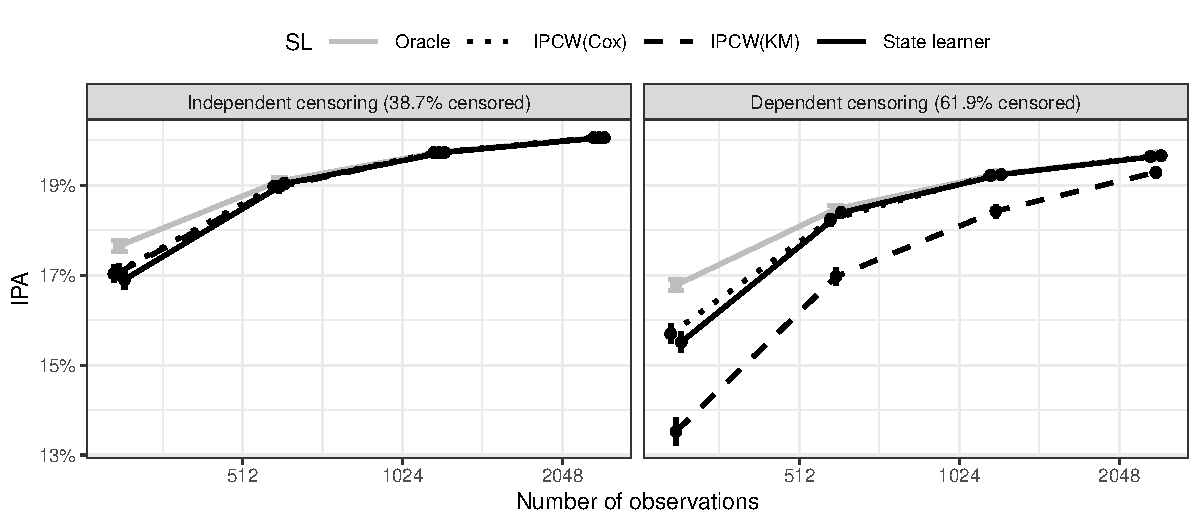
\includegraphics[width=1\linewidth]{experiment-fig-sl-ipcw.pdf}
  \caption[]{For the risk prediction models provided by each of the super
    learners, the IPA is plotted against sample size. The results are averages across 
    1000 simulated data sets and the error bars are used to quantify the Monte Carlo
    uncertainty.
  }
  \label{fig:ipcw-fail}
\end{figure}

We next compare the state learner to the super learner \texttt{survSL}
\citep{westling2021inference}. This is another super learner which
like the state learner works without a pre-specified censoring
model. Note that both the state learner and \texttt{survSL} provide a
prediction model for the event time outcome and also for the
probability of being censored. Hence, we compare the performance of
these methods with respect to both the outcome and the censoring
distribution. Again we use the IPA to quantify the predictive
performance.

The results are shown in Figures~\ref{fig:zelefski-out}
and~\ref{fig:zelefski-cens}. We see that for most sample sizes, the state
learner selected prediction models for both censoring and outcome which have
similar or higher IPA compared to the prediction models selected by
\texttt{survSL}.
\begin{figure}
  \centering %
  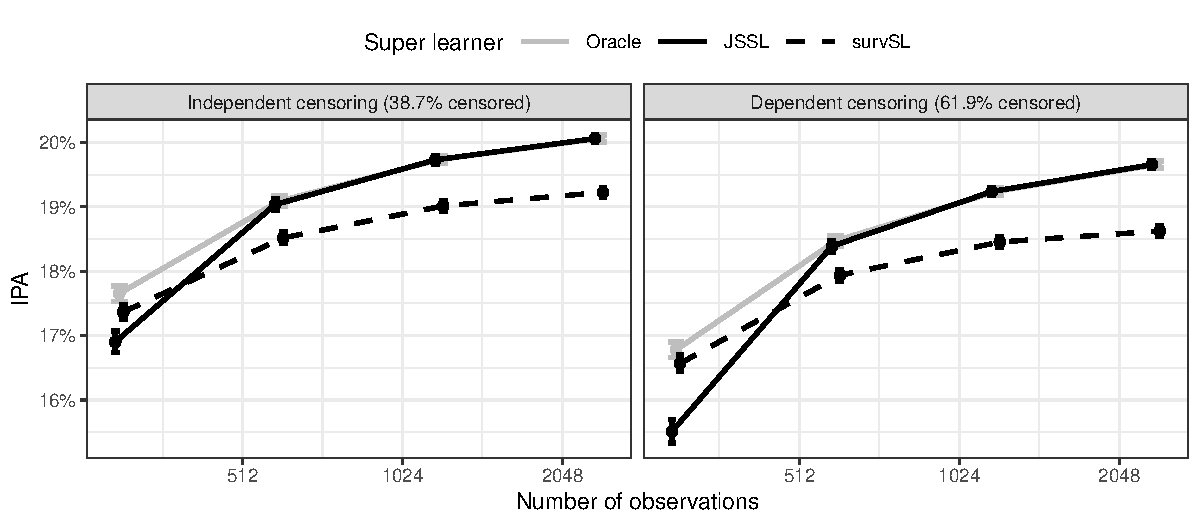
\includegraphics[width=1\linewidth]{experiment-fig-sl-survSL-out.pdf}
  \caption[]{For the risk prediction models of the outcome provided by each
    of the super learners, the IPA at the fixed time horizon is plotted against
    sample size. The results are averages across 1000 repetitions and the error
    bars are used to quantify the Monte Carlo uncertainty.}
  \label{fig:zelefski-out}
\end{figure}

\begin{figure}
  \centering %
  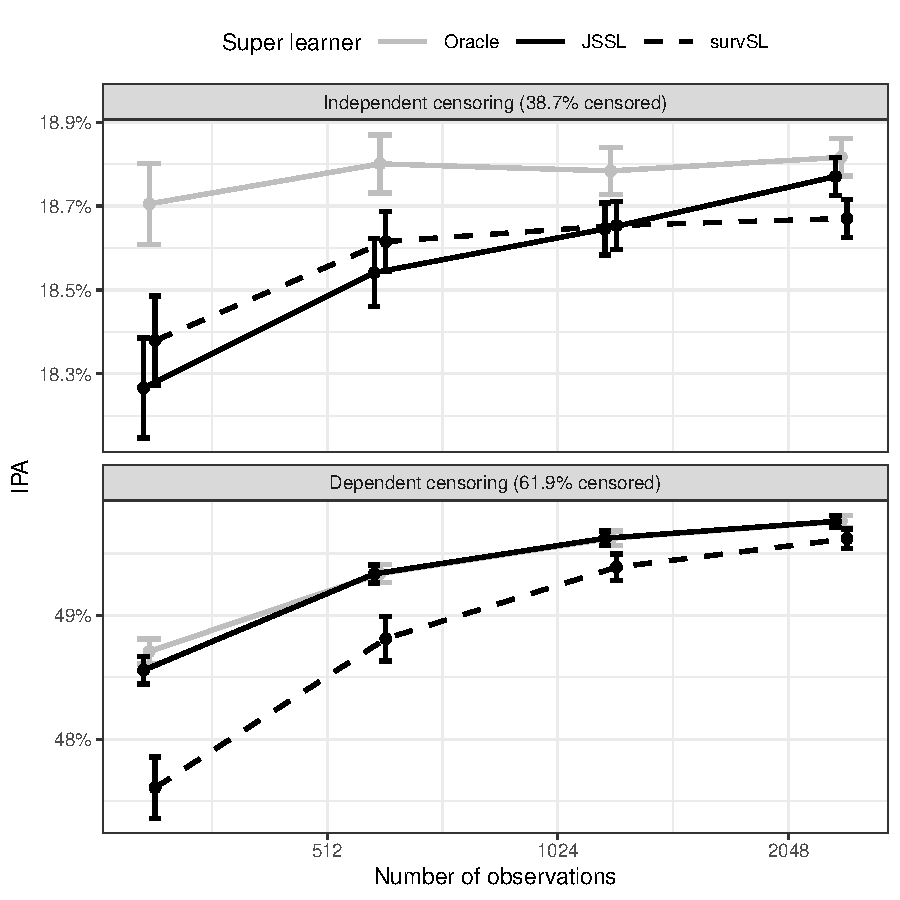
\includegraphics[width=.7\linewidth]{experiment-fig-sl-survSL-cens.pdf}
  \caption[]{For the risk prediction models of the censoring model provided by
    each of the super learners, the IPA at the fixed time horizon is plotted
    against sample size. The results are averages across 1000 repetitions and
    the error bars are used to quantify the Monte Carlo uncertainty.}
  \label{fig:zelefski-cens}
\end{figure}


\section{Prostate cancer study}
\label{sec:real-data-appl}

In this section we use the prostate cancer data of
\cite{kattan2000pretreatment} to illustrate the use of the state
learner in the presence of competing risks. We have introduced the
data in Section~\ref{sec:numer-exper}. The data consists of 1,042
patients who are followed from start of followup until tumor
recurrence, death without tumor recurrence or end of followup
(censored) whatever came first. For the sole purpose of illustration,
we estimate the average treatment effect of hormone therapy on death
and tumor recurrence. To do this we adapt the estimation strategy of
Section~\ref{sec:targeted-learning} as follows. We use the state
learner to rank libraries of learners for the cause-specific
cumulative hazard functions of tumor recurrence, death without tumor
recurrence, and censoring.  The libraries of learners each include
five learners: the Nelson-Aalen estimator, three Cox regression models
(unpenalized, Lasso, Elastic net) each including additive effects of
the 5 covariates (Section~\ref{sec:numer-exper}), and a random
survival forest. We use the same set of learners to learn the
cumulative hazard function of tumor recurrence \( \Lambda_1 \), the
cumulative hazard function of death without tumor recurrence
\( \Lambda_2 \), and the cumulative hazard function of the conditional
censoring distribution $\Gamma$.  We then use the highest ranked
combination of learners and apply
formula~\eqref{eq:one-step-comp-ate}.

This gives a library consisting of \( 5^3 = 125 \) learners for the
conditional state occupation probability function \( F \) defined in
equation~(\ref{eq:F-def}). We use five folds for training and testing
the models, and we repeat training and evaluation five times with
different splits.  The integrated Brier score (defined in
Section~\ref{sec:super-learner-simple}) for all learners are shown in
Figure~\ref{fig:zelefski-real}. We see that the prediction
performance is mostly affected by the choice of learner for the
censoring distribution. Several combinations of learners give similar
performance as measured by the integrated Brier score, as long as a
random forest is used to model the censoring distribution.

\begin{figure}
  \centering %
  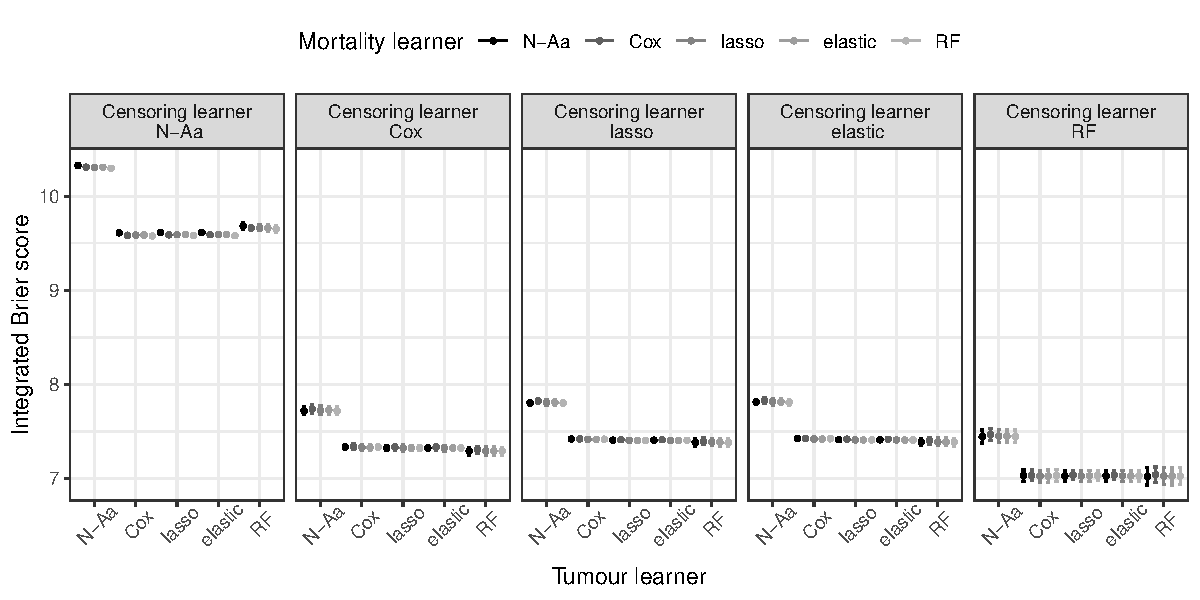
\includegraphics[width=1\linewidth]{real-data-state-learner.pdf}
  \caption[]{The results of applying the 125 combinations of learners to the
    prostate cancer data set. The error bars are based on five repetitions using
    different splits. We refer to learners of \( \Lambda_1 \), \( \Lambda_2 \),
    and $\Gamma$ as `Tumor learner', `Mortality learner', and `Censoring
    learner', respectively.}
  \label{fig:zelefski-real}
\end{figure}


We use the learners of the three cumulative hazard functions selected
by the state learner and the estimator defined in
Section~\ref{sec:cause-spec-aver},
equation~(\ref{eq:one-step-comp-ate}), to estimate the average
treatment effect of hormone therapy on risk of tumor recurrence and
death. The propensity score is estimated with a lasso model that
includes all levels of interaction.
The results are shown in Figure~\ref{fig:zelefski-real-target} for 6
month intervals after baseline with pointwise 95\% confidence
intervals. We see that hormone therapy decreases the risk of tumor
recurrence and increases the risk of death without tumor recurrence,
but that none of the estimated effects are statistically significant.

\begin{figure}
  \centering%
  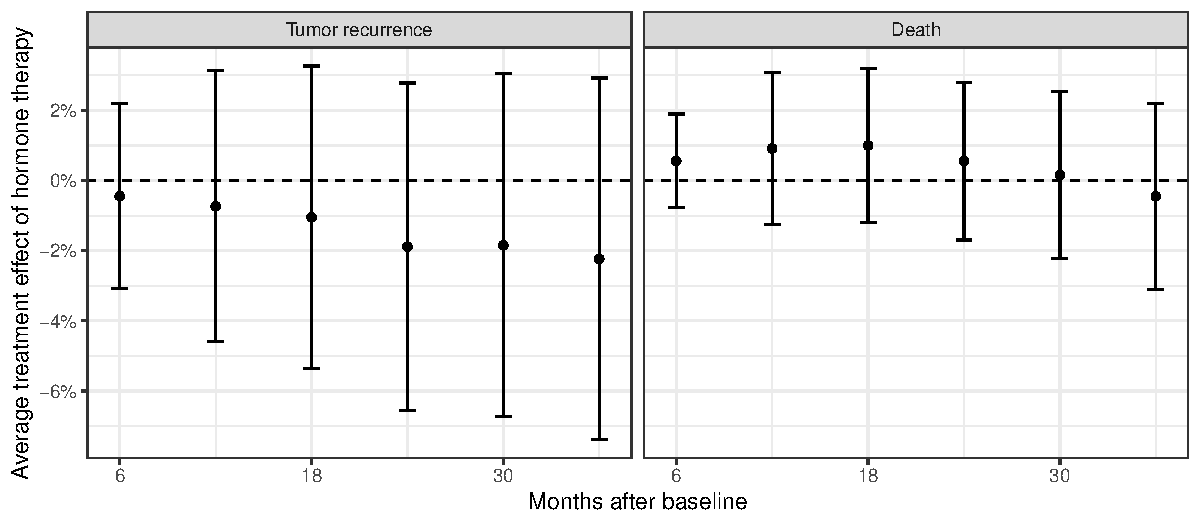
\includegraphics[width=1\linewidth]{real-data-target.pdf}
  \caption[]{Estimates of the average treatment effect of hormone therapy on the
    risk of tumor recurrence and death obtained from the prostate cancer study
    analysed by \cite{kattan2000pretreatment}. The estimates are based on the
    estimator defined in equation~(\ref{eq:one-step-comp-ate}) with pointwise
    95\% confidence intervals calculated as described in
    Section~\ref{sec:targeted-learning}. The estimates of the nuisance
    parameters are provided by the state learner.}
  \label{fig:zelefski-real-target}
\end{figure}



\section{Discussion}
\label{sec:discussion}

The state learner is a new super learner that can be used with
right-censored data and competing events. Compared to existing
IPCW-based methods, the advantage of the state learner is that it does
not depend on a pre-specified estimator of the censoring distribution,
but selects one automatically based on a library of learners for the
censoring distribution. Furthermore, the state learner neither
requires that the cause-specific cumulative hazard functions
\( \Lambda_j \) can be written as integrals with respect to Lebesgue
measure, nor does it assume a (semi-)parametric formula. In the
remainder of this section we discuss the limitations of our proposal
and avenues for further research.

A major advantage of the state learner is that the performance of each
combination of learners can be estimated without additional nuisance
parameters. A potential drawback of our approach is that we are
evaluating the loss of the learners on the level of the observed data
distribution while the target of the analysis is either the event time
distribution, or the censoring distribution, or both.
Specifically, the finite sample oracle inequality in
Corollary~\ref{cor:oracle-prop} concerns the function \( F \), which
is a feature of \( P \in \mathcal{P} \), while what we are typically
interested in is \( \Lambda_j \) or \( S \), which are features of
\( Q \in \mathcal{Q} \). We emphasise that while the state learner
provides us with estimates of \( \Lambda_j \) and $\Gamma$ based on
libraries \( \mathcal{A}_j \) and \( \mathcal{B} \), the performance
of these learners is not assessed directly for their respective target
parameters, but only indirectly via the performance of \( F \).  For
settings without competing risks, our numerical studies suggest that
measuring the performance of \( F \) also leads to good performance
for estimation of \( S \).

Our proposed super learner can be implemented with a broad library of learners
and using existing software.
% For instance the \texttt{R}-package
% \texttt{riskRegression} \citep{Gerds_Ohlendorff_Ozenne_2023} and the \texttt{R}-package by westling
Furthermore, while
the library \( \mathcal{F}(\mathcal{A}_1,\mathcal{A}_2,\mathcal{B}) \) consists
of \( |\mathcal{A}_1||\mathcal{A}_2||\mathcal{B}| \) many learners, we only need to fit
\( |\mathcal{A}_1| +|\mathcal{A}_2| + |\mathcal{B}| \) many learners in each fold. To
evaluate the performance of each learner we need to perform
\( |\mathcal{A}_1||\mathcal{A}_2||\mathcal{B}| \) many operations to calculate the
integrated Brier score in each hold-out sample, one for each combination of the
fitted models, but these operations are often negligible compared to fitting the
models. Hence the state learner is essentially not more computationally demanding
than any procedure that uses super learning to learn $\Lambda_1$, $\Lambda_2$,
and $\Gamma$ separately. While our proposal is based on constructing the library
\( \mathcal{F} \) from libraries for learning \( \Lambda_1 \), $\Lambda_2$, and
$\Gamma$, it could also be of interest to consider learners that estimate
\( F \) directly.

In our numerical studies, we only considered learners of $\Lambda_j$ and
$\Gamma$ that provide cumulative hazard functions which are piece-wise constant
in the time argument. This simplifies the calculation of \( F \) as the
integrals in equation~(\ref{eq:transition}) reduce to sums. When $\Lambda_j$ or
\( \Gamma \) are absolutely continuous in the time argument, calculating \( F \)
is more involved, but we expect that a good approximation can be achieved by
discretisation.

\section*{Conflict of interest}

The authors declare that they have no conflict of interest.


% BibTeX users please use one of
% \bibliographystyle{spbasic}      % basic style, author-year citations
%\bibliographystyle{spmpsci}      % mathematics and physical sciences
%\bibliographystyle{spphys}       % APS-like style for physics

\bibliographystyle{abbrvnat}
\bibliography{bib.bib}   % name your BibTeX data base

\appendix

\section{Proofs}
\label{sec:proofs}

This section contains proofs of the results stated in the paper.
Section~\ref{sec:consistency-proof} contains a proof of the consistency result
from Section~\ref{sec:consistency}; Section~\ref{sec:oracle-inequalities}
contains proofs of the oracle inequalities from
Section~\ref{sec:finite-sample-oracle}; and
Section~\ref{sec:state-learner-with} demonstrates transience of the second
order remainder structure stated in Section~\ref{sec:trans-second-order}.

\subsection{Consistency}
\label{sec:consistency-proof}

Define
\( \bar{B}_{\tau,0}(F, o) = \bar{B}_{\tau}(F, o) - \bar{B}_{\tau}(F_0, o) \) and
\( R_{0}(F) = P_0{[\bar{B}_{\tau,0}(F, \blank)]} \), where the integrated Brier
score \( \bar{B}_{\tau} \) was defined in
Section~\ref{sec:super-learner-simple}.
\begin{lemma}
  \label{lemma:norm}
  \( R_{0}(F) = \Vert F - F_0 \Vert_{P_0}^2 \), where \( \Vert \blank \Vert_{P_0}\) is defined
  in equation~(\ref{eq:norm}).
\end{lemma}
\begin{proof}[Proof]
  For any \( t \in [0, \tau] \) and \( j\in \{-1,0,1,2\} \) we have
  \begin{align*}
    & \E_{P_0}{\left[ (F(t, j, X) - \1{\{\eta(t) = j \}})^2 \right]}
    \\
    & =    \E_{P_0}{\left[ (F(t, j, X) - F_0(t, j, X) + F_0(t, j, X) - \1{\{\eta(t) = j
      \}})^2 \right]}
    \\
    & =    \E_{P_0}{\left[ (F(t, j, X) - F_0(t, j, X))^2\right]}
      + \E_{P_0}{\left[ (F_0(t, j, X) - \1{\{\eta(t) = j \}})^2\right]}
    \\
    & \quad
      + 2\E_{P_0}{\left[ (F(t, j, X) - F_0(t, j, X))(F_0(t, j, X) - \1{\{\eta(t) = j
      \}})\right]}
    \\
    & =    \E_{P_0}{\left[ (F(t, j, X) - F_0(t, j, X))^2\right]}
      + \E_{P_0}{\left[ (F_0(t, j, X) - \1{\{\eta(t) = j \}})^2\right]},
  \end{align*}
  where the last equality follows from the tower property. Hence, using Fubini,
  we have
  \begin{equation*}
    P{[\bar{B}_{\tau}(F, \blank)]}
    = \Vert F - F_0 \Vert_{P_0}^2 + P_0{[\bar{B}_{\tau}(F_0, \blank)]}.
  \end{equation*}
\end{proof}

\begin{proof}[Proof of Proposition~\ref{prop:stric-prop}]
  The result follows from Lemma~\ref{lemma:norm}.
\end{proof}

\subsection{Oracle inequalities}
\label{sec:oracle-inequalities}

Recall that we use \( \mathcal{F}_n \) to denote a library of learners for the
function \( F \), and that \( \hat{\phi} \) and \( \tilde{\phi} \) denotes,
respectively, the discrete super learner and the oracle learner for the library
\( \mathcal{F}_n \), c.f., Section~\ref{sec:super-learner-simple}.

\begin{proof}[Proof of Corollary~\ref{cor:oracle-prop}]
  First note that minimising the loss \( \bar{B}_{\tau} \) is equivalent to
  minimising the loss \( \bar{B}_{\tau,0} \), so the discrete super learner and
  oracle according to \( \bar{B}_{\tau} \) and \( \bar{B}_{\tau,0} \) are
  identical. By Lemma~\ref{lemma:norm}, \( R_0(F) \geq 0 \) for any
  \( F \in \mathcal{H}_{\mathcal{P}} \), and so using Theorem 2.3 from
  \citep{vaart2006oracle} with \( p=1 \), we have that for all \( \delta >0 \),
\begin{align*}
  & \E_{P_0}{\left[ R_0(\hat{\phi}_n(\data_n^{-k})) \right]}
  \\
  &  \quad \leq
    (1+2\delta)\E_{P_0}{\left[ R_0(\tilde{\phi}_n(\data_n^{-k})) \right]}
  \\
  & \qquad + (1+\delta) \frac{16 K}{n}
    \log(1 + |\mathcal{F}_n|)\sup_{F \in \mathcal{H}_{\mathcal{P}}}
    \left\{
    M(F) + \frac{v(F)}{R_0(F)}
    \left(
    \frac{1}{\delta} + 1
    \right)
    \right\}
\end{align*}
where for each \( F \in \mathcal{H}_{\mathcal{P}} \), \( (M(F), v(F)) \) is some Bernstein pair for
the function \(o \mapsto \bar{B}_{\tau,0}(F, o) \). As
\( \bar{B}_{\tau,0}(F, \blank) \) is uniformly bounded by \( \tau \) for any
\( F \in \mathcal{H}_{\mathcal{P}} \), it follows from section 8.1 in \citep{vaart2006oracle} that
\( (\tau, 1.5 P_0{[\bar{B}_{\tau,0}(F, \blank)^2]}) \) is a Bernstein pair for
\( \bar{B}_{\tau,0}(F, \blank) \). Now, for any \( a,b,c \in \R \) we have
\begin{align*}
  (a-c)^2 - (b-c)^2
  & = (a-b+b-c)^2 - (b-c)^2
  \\
  & = (a-b)^2 + (b-c)^2 +2(b-c)(a-b) - (b-c)^2
  \\
  & = (a-b)
    \left\{
    (a-b) +  2(b-c)
    \right\}
  \\
  & = (a-b)
    \left\{
     a + b -2c
    \right\},
\end{align*}
so using this with \( a=F(t, j, x) \), \( b=F_0(t, j, x) \), and
\( c = \1{\{\eta(t) = j\}} \), we have by Jensen's inequality
\begin{align*}
  & P_0{[\bar{B}_{\tau,0}(F, \blank)^2]}
  \\
  & \leq
    2\tau\E_{P_0}{\left[
    \sum_{j=-1}^{2} \int_0^{\tau}
    \left\{
    \left(
    F(t, j, X) - \1{\{\eta(t) = j\}}
    \right)^2
    -
    \left(
    F_0(t, j, X) - \1{\{\eta(t) = j\}}
    \right)^2
    \right\}^2
    \diff t 
    \right]}
  \\
  & =2\tau
    \E_{P_0}\Bigg[
    \sum_{j=-1}^{2} \int_0^{\tau}
    \left(
    F(t, j, X) - F_0(t, j, X)
    \right)^2
  \\
  & \quad \quad \quad\quad \quad \quad \times
    \left\{
    F(t, j, X) +  F_0(t, j, X)-2 \1{\{\eta(t) = j\}}
    \right\}^2
    \diff t 
    \Bigg]
  \\
  & \leq
    8\tau \E_{P_0}{\left[
    \sum_{j=-1}^{2} \int_0^{\tau}
    \left(
    F(t, j, X) - F_0(t, j, X)
    \right)^2
    \diff t 
    \right]}.
  \\
  & =
    8\tau \Vert F - F_0 \Vert_{P_0}^2.
\end{align*}
Thus when \( v(F) = 1.5 P_0{[\bar{B}_{\tau,0}(F, \blank)^2]} \) we have by
Lemma~\ref{lemma:norm}
\begin{equation*}
  \frac{v(F)}{R_0(F)}
  = 1.5 \frac{P_0{[\bar{B}_{\tau,0}(F, \blank)^2]}}{P_0{[\bar{B}_{\tau,0}(F, \blank)]}}
  \leq 12 \tau,
\end{equation*}
and so using the Bernstein pairs \( (\tau, 1.5 P_0{[\bar{B}_{\tau,0}(F, \blank)^2]}) \) we have
\begin{equation*}
  \sup_{F \in \mathcal{H}_{\mathcal{P}}}
  \left\{
    M(F) + \frac{v(F)}{R_0(F)}
    \left(
      \frac{1}{\delta} + 1
    \right)
  \right\}
  \leq \tau
  \left(
    13 + \frac{12}{\delta}
  \right),
\end{equation*}
For all $\delta>0$ we thus have
\begin{align*}
  \E_{P_0}{\left[ R_0(\hat{\phi}_n(\data_n^{-k})) \right]}
  \leq
  &(1+2\delta)\E_{P_0}{\left[ R_0(\tilde{\phi}_n(\data_n^{-k})) \right]}
  \\
  & \quad
    + (1+\delta)\log(1 + |\mathcal{F}_n|) \tau \frac{16 K}{n}
    \left(
    13 + \frac{12}{\delta}
    \right),
\end{align*}
and then the final result follows from Lemma~\ref{lemma:norm}.
\end{proof}

\begin{proof}[Proof of Corollary~\ref{cor:asymp-cons}]
  By definition of the oracle and Lemma~\ref{lemma:norm},
  \begin{equation*}
    \E_{P_0}{\left[ \Vert \tilde{\phi}_n(\data_n^{-k}) - F_0 \Vert_{P_0}^2
      \right]} \leq \E_{P_0}{\left[ \Vert \phi_n(\data_n^{-k}) - F_0 \Vert_{P_0}^2
      \right]}  
  \end{equation*}
  for all \( n \in \N \). The results then follows from
  Corollary~\ref{cor:oracle-prop}.
\end{proof}


\subsection{Transience of the second order remainder structure}
\label{sec:state-learner-with}

Recall that we let $\Lambda_1$ denote the conditional cumulative hazard function
for one of the event times of interest and $\Gamma$ the conditional cumulative
hazard function for censoring, c.f., Section~\ref{sec:framework}.

\begin{proof}[Proof of Proposition~\ref{prop:dr-structure}]
  For notational convenience we suppress \( X \) in the following. The final
  result can be obtained by adding the argument \( X \) to all functions and
  averaging. We use the relations from equation~\eqref{eq:7} to write
  \begingroup %
  \allowdisplaybreaks
    \begin{align*}
      & \int_0^{\tau} w(s) 
        \left\{
        \Gamma(s) - \hat{\Gamma}_n(s)
        \right\}
        [\Lambda_1 - \hat{\Lambda}_{1,n}](\diff s)
      \\
      & =
        \int_0^{\tau} w(s) 
        \left\{
        \int_0^s \frac{F(\diff u, -1)}{F(u-, 0)} -
        \int_0^s \frac{\hat{F}_n(\diff u, -1)}{\hat{F}_n(u-, 0)}  -
        \right\}
        \left[
        \frac{F(\diff s, 1)}{F(s-, 0)}
        - \frac{\hat{F}_n(\diff s, 1)}{\hat{F}_n(s-, 0)}
        \right]
      \\
      & =
        \int_0^{\tau} w(s) 
        \Bigg\{
        \int_0^s 
        \left(
        \frac{1}{F(u-, 0)} -  \frac{1}{\hat{F}_n(u-, 0)}
        \right) F(\diff u, -1)
      \\
      & \qquad\qquad \qquad
        +
        \int_0^s \frac{1}{\hat{F}_n(u-, 0)} 
        \left[
        F(\diff u, -1) - \hat{F}_n(\diff u, -1)
        \right]
        \Bigg\}
      \\
      & \qquad\qquad \times
        \left[
        \left(
        \frac{1}{F(s-, 0)} -
        \frac{1}{\hat{F}_n(s-, 0)}
        \right)F(\diff s, 1)
        + \frac{1}{\hat{F}_n(s-, 0)}
        \left(
        F(\diff s, 1) -
        \hat{F}_n(\diff s, 1)
        \right)
        \right]
      \\
      &
        = \int_0^{\tau} 
        \int_0^s
        w(s) 
        \left(
        \frac{1}{F(u-, 0)} -  \frac{1}{\hat{F}_n(u-, 0)}
        \right) 
        \left(
        \frac{1}{F(s-, 0)} -
        \frac{1}{\hat{F}_n(s-, 0)}
        \right)F(\diff u, -1)F(\diff s, 1)
      \\
      & \quad +
        \int_0^{\tau}
        \int_0^s
        w(s) 
        \left(
        \frac{1}{F(u-, 0)} -  \frac{1}{\hat{F}_n(u-, 0)}
        \right) \frac{F(\diff u, -1) }{\hat{F}_n(u-,0)}
        \left(
        F(\diff s, 1) -
        \hat{F}_n(\diff s, 1)
        \right)
      \\
      & \quad +
        \int_0^{\tau} 
        \int_0^s      
        \frac{w(s) }{\hat{F}_n(u-, 0)} 
        \left[
        F(\diff u, -1) - \hat{F}_n(\diff u, -1)
        \right]
        \left(
        \frac{1}{F(s-, 0)} -
        \frac{1}{\hat{F}_n(s-, 0)}
        \right)F(\diff s, 1)
      \\
      & \quad +
        \int_0^{\tau} 
        \int_0^s      
        \frac{w(s) }{\hat{F}_n(u-, 0)} 
        \left[
        F(\diff u, -1) - \hat{F}_n(\diff u, -1)
        \right]
        \frac{1}{\hat{F}_n(s-, 0)}
        \left(
        F(\diff s, 1) -
        \hat{F}_n(\diff s, 1)
        \right).
    \end{align*}
    \endgroup %
    Consider the first term on the right hand side. By the mean value theorem,
    \begin{equation*}
      \frac{1}{F(t-, 0)}
      - \frac{1}{\hat{F}_n(t-, 0)}
      = \frac{-1}{\tilde{r}_n(t)^2}
      \left[
        F(t-, 0)
        - \hat{F}_n(t-, 0)
      \right],
    \end{equation*}
    where \( \tilde{r}_n(t) \) is some value between \( \hat{F}(t-, 0) \) and
    \( \hat{F}_n(t-, 0) \). Letting \( w_n^*(t) = -\tilde{r}_n(t)^{-2} \), we
    may write
  \begin{align*}
    & \int_0^{\tau} 
      \int_0^s
      w(s) 
      \left(
      \frac{1}{F(u-, 0)} -  \frac{1}{\hat{F}_n(u-, 0)}
      \right)      
      \left(
      \frac{1}{F(s-, 0)} -
      \frac{1}{\hat{F}_n(s-, 0)}
      \right)F(\diff u, -1)F(\diff s, 1)
    \\
    & =
      \int_0^{\tau} 
      \int_0^s
      w(s)
      w_n^*(u) 
      \left(
      F(u-, 0) - \hat{F}_n(u-, 0)
      \right)
    \\
    & \qquad \qquad \quad
      \times
      w_n^*(s) 
      \left(
      F(s-, 0) - \hat{F}_n(s-, 0)
      \right)       
      F(\diff u, -1)F(\diff s, 1)
    \\
    & =
      \int_0^{\tau} 
      \int_0^s
      w_n^a(s,u)
      \left(
      F(u-, 0) - \hat{F}_n(u-, 0)
      \right)
      \left(
      F(s-, 0) - \hat{F}_n(s-, 0)
      \right)       
      F(\diff u, -1)F(\diff s, 1),
  \end{align*}
  where we have defined \( w_n^a(s,u) = w(s)w^*_n(s)w^*_n(u) \). By the
  assumption that \( F(\blank,0) \) and \( F_n(\blank,0) \) are uniformly
  bounded away from zero on \( [0,\tau] \), it follows that \( w_n^* \) is
  uniformly bounded, and hence \( w_n^a(s,u) \) is also uniformly bounded,
  because \( w \) was assumed uniformly bounded. The same approach can be
  applied to the three remaining terms which gives the result.
\end{proof}


\end{document}
% end of file template.tex

